% !TEX root = ./main.tex
% Basic Blocks and Traces
% ======================================================
\par \noindent Canonical Form 特征:所有语句都被带到树的顶层、可以直接生成汇编。定义:
1. 没有 \texttt{SEQ} 或 \texttt{ESEQ}:规范树中的根节点是唯一的 stmt(如 \texttt{MOVE} 或 \texttt{EXP} ),
而其他节点都是 expr(如 \texttt{BINOP}、\texttt{MEM} 等),这样保证了树的结构更加简洁和明确;
2. 每个 \texttt{CALL} 节点的父节点要么是 \texttt{EXP(...)} 节点,要么是 \texttt{MOVE(TEMP t, ...)} 节点:
\texttt{CALL} 节点不能嵌套在其他表达式中,必须直接成为根节点的子节点,同时,根节点必须是上述两者之一,
这样设计是为了确保 \texttt{CALL} 的副作用(例如修改全局状态)能够被明确控制和管理。

\par \noindent stmt 和 expr 的可交换性:
如果 s 不影响 e 的值,则 s 和 e 是可交换的。例如,如果 \texttt{t1 != t2},那么 stmt \texttt{MOVE (MEM(t1), e)} 和 \texttt{MEM(t2)} 是可交换的。
如果不可交换,需要新的临时变量来存储中间结果。
问题:为什么 \texttt{BINOP(op, ESEQ(s, e1), e2)} 转换为 \texttt{ESEQ(S, BINOP(op, e1e2))} 不需要考虑 s 和 e2 的可交换性,
而 \texttt{BINOP(op, e1, ESEQ(S, e2))} 则要考虑 s 和 e1 的可交换性?
这是因为 \texttt{BINOP(op, e1, e2)} 对 e1 和 e2 的运算顺序是从左往右计算的。
对于第一种情况,考虑 s 的影响在求值 e1 和 e2 之前。
而对于第二种情况,考虑 s 的影响则是在求值 e1 和 e2 之间,就可能会出现 s 实际上只影响 e2 但没有影响 e1,
但如果直接提升 \texttt{ESEQ} 至 \texttt{BINOP} 外侧,则 s 非预期地同时影响了 e1 和 e2 的值。

\par \noindent 有关 \texttt{CALL} 的变换:\texttt{CALL(fun, args)} $\rightarrow$ \texttt{ESEQ(MOVE(TEMP t, CALL(fun, args)), TEMP t)}。

\par \noindent 有关 \texttt{SEQ} 的变换:\texttt{SEQ(SEQ(a, b), c)} $\rightarrow$ \texttt{SEQ(a, seq(b, c))}。

\par \noindent 有关 \texttt{ESEQ} 的变换(不全,Tiger Ex. 8.1):

\begin{figure}[H]
    \centering
    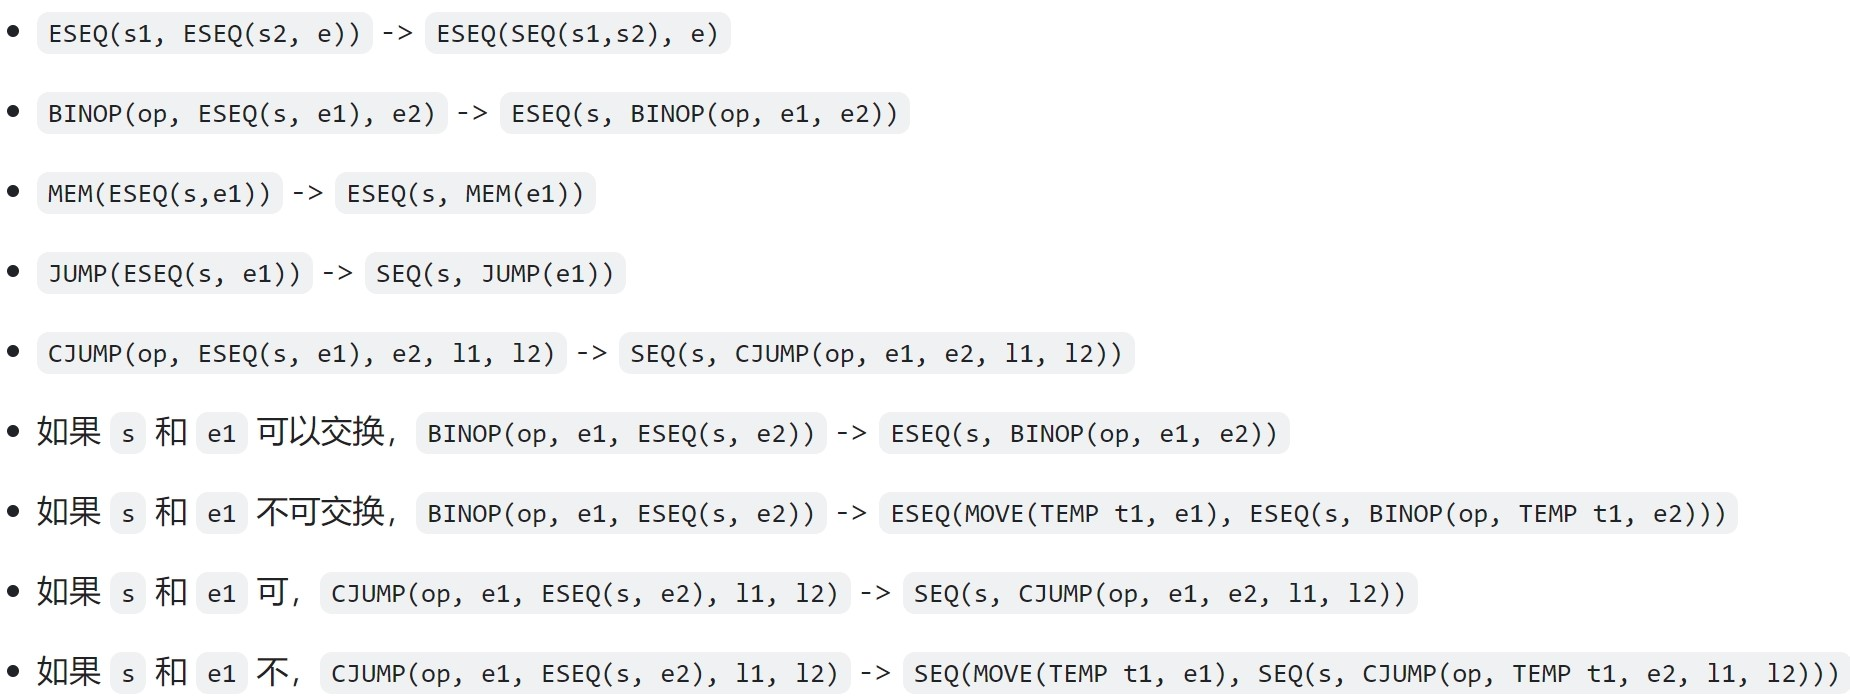
\includegraphics[width=\linewidth]{figures/irc1.png}
\end{figure}

\par \noindent Basic Blocks:一段代码中,只有一个入口点和一个出口点的连续代码块。Trace: 可以连续执行的基本块序列。
计算 trace:1. 某个 basic block 开始,往后继节点遍历,标记每个被访问的 basic block 并将其附加到当前 trace 中;
2. 当到达某 basic block 其后继节点均已标记,这个 trace 就算完了。
计算新的 trace:选择一个未标记的 basic block 作为下一个 trace 的起点。
全局终止条件:不断迭代、 直到所有的 basic blocks 都被标记。
(性质)每个 trace 都是无环的。

\par \noindent 调整 \texttt{CJUMP} 后面紧跟的标签:a. 如果跟着的标签是 true 标签,互换 true 和 false 标签,并对条件取反;
b. 如果跟着的标签是 false 标签,什么都不做;
c. 如果跟着的标签既不是 true 标签,也不是 false 标签,替换 \texttt{CJUMP(cond, a, b, lt, lf)} $\rightarrow$
\texttt{CJUMP(cond, a, b, lt, lf'); LABEL lf'; JUMP(NAME lf)}。